\PassOptionsToPackage{unicode=true}{hyperref} % options for packages loaded elsewhere
\PassOptionsToPackage{hyphens}{url}
%
\documentclass[
  10pt,
  ignorenonframetext,
]{beamer}
\usepackage{pgfpages}
\setbeamertemplate{caption}[numbered]
\setbeamertemplate{caption label separator}{: }
\setbeamercolor{caption name}{fg=normal text.fg}
\beamertemplatenavigationsymbolsempty
% Prevent slide breaks in the middle of a paragraph:
\widowpenalties 1 10000
\raggedbottom
\setbeamertemplate{part page}{
  \centering
  \begin{beamercolorbox}[sep=16pt,center]{part title}
    \usebeamerfont{part title}\insertpart\par
  \end{beamercolorbox}
}
\setbeamertemplate{section page}{
  \centering
  \begin{beamercolorbox}[sep=12pt,center]{part title}
    \usebeamerfont{section title}\insertsection\par
  \end{beamercolorbox}
}
\setbeamertemplate{subsection page}{
  \centering
  \begin{beamercolorbox}[sep=8pt,center]{part title}
    \usebeamerfont{subsection title}\insertsubsection\par
  \end{beamercolorbox}
}
\AtBeginPart{
  \frame{\partpage}
}
\AtBeginSection{
  \ifbibliography
  \else
    \frame{\sectionpage}
  \fi
}
\AtBeginSubsection{
  \frame{\subsectionpage}
}
\usepackage{lmodern}
\usepackage{amssymb,amsmath}
\usepackage{ifxetex,ifluatex}
\ifnum 0\ifxetex 1\fi\ifluatex 1\fi=0 % if pdftex
  \usepackage[T1]{fontenc}
  \usepackage[utf8]{inputenc}
  \usepackage{textcomp} % provides euro and other symbols
\else % if luatex or xelatex
  \usepackage{unicode-math}
  \defaultfontfeatures{Scale=MatchLowercase}
  \defaultfontfeatures[\rmfamily]{Ligatures=TeX,Scale=1}
\fi
\usetheme[]{Dresden}
\usecolortheme{dolphin}
\usefonttheme{structuresmallcapsserif}
% use upquote if available, for straight quotes in verbatim environments
\IfFileExists{upquote.sty}{\usepackage{upquote}}{}
\IfFileExists{microtype.sty}{% use microtype if available
  \usepackage[]{microtype}
  \UseMicrotypeSet[protrusion]{basicmath} % disable protrusion for tt fonts
}{}
\makeatletter
\@ifundefined{KOMAClassName}{% if non-KOMA class
  \IfFileExists{parskip.sty}{%
    \usepackage{parskip}
  }{% else
    \setlength{\parindent}{0pt}
    \setlength{\parskip}{6pt plus 2pt minus 1pt}}
}{% if KOMA class
  \KOMAoptions{parskip=half}}
\makeatother
\usepackage{xcolor}
\IfFileExists{xurl.sty}{\usepackage{xurl}}{} % add URL line breaks if available
\IfFileExists{bookmark.sty}{\usepackage{bookmark}}{\usepackage{hyperref}}
\hypersetup{
  pdftitle={Machine Learning - Solution/Exercises},
  pdfauthor={Jan-Philipp Kolb},
  pdfborder={0 0 0},
  breaklinks=true}
\urlstyle{same}  % don't use monospace font for urls
\newif\ifbibliography
\usepackage{color}
\usepackage{fancyvrb}
\newcommand{\VerbBar}{|}
\newcommand{\VERB}{\Verb[commandchars=\\\{\}]}
\DefineVerbatimEnvironment{Highlighting}{Verbatim}{commandchars=\\\{\}}
% Add ',fontsize=\small' for more characters per line
\newenvironment{Shaded}{}{}
\newcommand{\AlertTok}[1]{\textcolor[rgb]{1.00,0.00,0.00}{#1}}
\newcommand{\AnnotationTok}[1]{\textcolor[rgb]{0.00,0.50,0.00}{#1}}
\newcommand{\AttributeTok}[1]{#1}
\newcommand{\BaseNTok}[1]{#1}
\newcommand{\BuiltInTok}[1]{#1}
\newcommand{\CharTok}[1]{\textcolor[rgb]{0.00,0.50,0.50}{#1}}
\newcommand{\CommentTok}[1]{\textcolor[rgb]{0.00,0.50,0.00}{#1}}
\newcommand{\CommentVarTok}[1]{\textcolor[rgb]{0.00,0.50,0.00}{#1}}
\newcommand{\ConstantTok}[1]{#1}
\newcommand{\ControlFlowTok}[1]{\textcolor[rgb]{0.00,0.00,1.00}{#1}}
\newcommand{\DataTypeTok}[1]{#1}
\newcommand{\DecValTok}[1]{#1}
\newcommand{\DocumentationTok}[1]{\textcolor[rgb]{0.00,0.50,0.00}{#1}}
\newcommand{\ErrorTok}[1]{\textcolor[rgb]{1.00,0.00,0.00}{\textbf{#1}}}
\newcommand{\ExtensionTok}[1]{#1}
\newcommand{\FloatTok}[1]{#1}
\newcommand{\FunctionTok}[1]{#1}
\newcommand{\ImportTok}[1]{#1}
\newcommand{\InformationTok}[1]{\textcolor[rgb]{0.00,0.50,0.00}{#1}}
\newcommand{\KeywordTok}[1]{\textcolor[rgb]{0.00,0.00,1.00}{#1}}
\newcommand{\NormalTok}[1]{#1}
\newcommand{\OperatorTok}[1]{#1}
\newcommand{\OtherTok}[1]{\textcolor[rgb]{1.00,0.25,0.00}{#1}}
\newcommand{\PreprocessorTok}[1]{\textcolor[rgb]{1.00,0.25,0.00}{#1}}
\newcommand{\RegionMarkerTok}[1]{#1}
\newcommand{\SpecialCharTok}[1]{\textcolor[rgb]{0.00,0.50,0.50}{#1}}
\newcommand{\SpecialStringTok}[1]{\textcolor[rgb]{0.00,0.50,0.50}{#1}}
\newcommand{\StringTok}[1]{\textcolor[rgb]{0.00,0.50,0.50}{#1}}
\newcommand{\VariableTok}[1]{#1}
\newcommand{\VerbatimStringTok}[1]{\textcolor[rgb]{0.00,0.50,0.50}{#1}}
\newcommand{\WarningTok}[1]{\textcolor[rgb]{0.00,0.50,0.00}{\textbf{#1}}}
\usepackage{graphicx,grffile}
\makeatletter
\def\maxwidth{\ifdim\Gin@nat@width>\linewidth\linewidth\else\Gin@nat@width\fi}
\def\maxheight{\ifdim\Gin@nat@height>\textheight\textheight\else\Gin@nat@height\fi}
\makeatother
% Scale images if necessary, so that they will not overflow the page
% margins by default, and it is still possible to overwrite the defaults
% using explicit options in \includegraphics[width, height, ...]{}
\setkeys{Gin}{width=\maxwidth,height=\maxheight,keepaspectratio}
\setlength{\emergencystretch}{3em}  % prevent overfull lines
\providecommand{\tightlist}{%
  \setlength{\itemsep}{0pt}\setlength{\parskip}{0pt}}
\setcounter{secnumdepth}{-2}

% set default figure placement to htbp
\makeatletter
\def\fps@figure{htbp}
\makeatother


\title{Machine Learning - Solution/Exercises}
\author{Jan-Philipp Kolb}
\date{27 Mai, 2019}

\begin{document}
\frame{\titlepage}

\begin{frame}[fragile]{\href{https://www.r-exercises.com/2016/12/13/recursive-partitioning-and-regression-trees-exercises/}{Exercise
- \texttt{rpart} Kyphosis}}
\protect\hypertarget{exercise---rpart-kyphosis}{}

\begin{block}{Consider the Kyphosis data frame}

\begin{enumerate}
[1)]
\tightlist
\item
  Which variables are in the \texttt{kyphosis} dataset
\item
  Build a tree to classify Kyphosis from Age, Number and Start.
\end{enumerate}

\end{block}

\begin{block}{Consider the tree build above.}

\begin{enumerate}
[1)]
\setcounter{enumi}{2}
\tightlist
\item
  Which variables are used to explain Kyphosis presence?
\item
  How many observations contain the terminal nodes.
\end{enumerate}

\end{block}

\begin{block}{Consider the Kyphosis data frame.}

\begin{enumerate}
[1)]
\setcounter{enumi}{4}
\tightlist
\item
  Build a tree using the first 60 observations of kyphosis.
\item
  Predict the kyphosis presence for the other 21 observations.
\item
  Which is the misclassification rate (prediction error)
\end{enumerate}

\end{block}

\end{frame}

\begin{frame}{\href{https://www.r-exercises.com/2016/12/13/recursive-partitioning-and-regression-trees-solutions/}{The
dataset kyphosis}}
\protect\hypertarget{the-dataset-kyphosis}{}

\begin{block}{The dataset contains (1):}

\begin{itemize}
\tightlist
\item
  Kyphosis: a factor with levels absent present indicating if a kyphosis
  (a type of deformation) was present after the operation.
\item
  Age: in months.
\item
  Number: the number of vertebrae involved.
\item
  Start: the number of the first (topmost) vertebra operated on.
\end{itemize}

\end{block}

\end{frame}

\begin{frame}[fragile]{Build the tree (2)}
\protect\hypertarget{build-the-tree-2}{}

\begin{Shaded}
\begin{Highlighting}[]
\KeywordTok{library}\NormalTok{(}\StringTok{'rpart'}\NormalTok{)}
\NormalTok{TREE <-}\StringTok{ }\KeywordTok{rpart}\NormalTok{(Kyphosis }\OperatorTok{~}\StringTok{ }\NormalTok{Age }\OperatorTok{+}\StringTok{ }\NormalTok{Number }\OperatorTok{+}\StringTok{ }\NormalTok{Start, }
              \DataTypeTok{data=}\NormalTok{kyphosis,}\DataTypeTok{method=}\StringTok{"class"}\NormalTok{)}
\NormalTok{TREE}
\end{Highlighting}
\end{Shaded}

\begin{verbatim}
## n= 81 
## 
## node), split, n, loss, yval, (yprob)
##       * denotes terminal node
## 
##  1) root 81 17 absent (0.79012346 0.20987654)  
##    2) Start>=8.5 62  6 absent (0.90322581 0.09677419)  
##      4) Start>=14.5 29  0 absent (1.00000000 0.00000000) *
##      5) Start< 14.5 33  6 absent (0.81818182 0.18181818)  
##       10) Age< 55 12  0 absent (1.00000000 0.00000000) *
##       11) Age>=55 21  6 absent (0.71428571 0.28571429)  
##         22) Age>=111 14  2 absent (0.85714286 0.14285714) *
##         23) Age< 111 7  3 present (0.42857143 0.57142857) *
##    3) Start< 8.5 19  8 present (0.42105263 0.57894737) *
\end{verbatim}

\end{frame}

\begin{frame}[fragile]{Plot the result}
\protect\hypertarget{plot-the-result}{}

\begin{Shaded}
\begin{Highlighting}[]
\KeywordTok{plot}\NormalTok{(TREE)}
\KeywordTok{text}\NormalTok{(TREE,}\DataTypeTok{use.n=}\NormalTok{T)}
\end{Highlighting}
\end{Shaded}

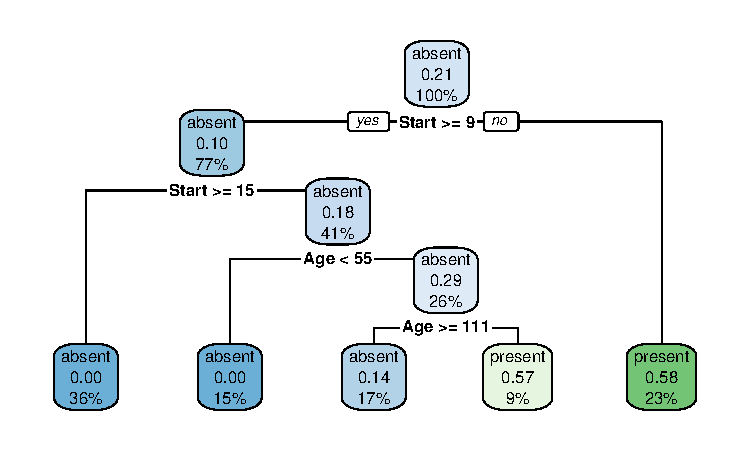
\includegraphics{ml_exercises_c1_treesbagging_files/figure-beamer/unnamed-chunk-2-1.pdf}

\end{frame}

\begin{frame}{Answers}
\protect\hypertarget{answers}{}

\begin{enumerate}
[1)]
\setcounter{enumi}{2}
\tightlist
\item
  Which variables are used to explain Kyphosis presence?
\end{enumerate}

\begin{itemize}
\tightlist
\item
  The variables are Start and Age
\end{itemize}

\begin{enumerate}
[1)]
\setcounter{enumi}{3}
\tightlist
\item
  How many observations contain the terminal nodes.
\end{enumerate}

\begin{itemize}
\tightlist
\item
  *denotes terminal nodes. The nodes have 29, 12, 14, 7 and 19
  observations
\end{itemize}

\end{frame}

\begin{frame}[fragile]{Consider the Kyphosis data frame.}
\protect\hypertarget{consider-the-kyphosis-data-frame.-1}{}

\begin{enumerate}
[1)]
\setcounter{enumi}{4}
\tightlist
\item
  Build a tree using the first 60 observations of kyphosis.
\end{enumerate}

\begin{Shaded}
\begin{Highlighting}[]
\NormalTok{TREE <-}\StringTok{ }\KeywordTok{rpart}\NormalTok{(Kyphosis }\OperatorTok{~}\StringTok{ }\NormalTok{Age }\OperatorTok{+}\StringTok{ }\NormalTok{Number }\OperatorTok{+}\StringTok{ }\NormalTok{Start, }
              \DataTypeTok{data=}\NormalTok{kyphosis[}\DecValTok{1}\OperatorTok{:}\DecValTok{60}\NormalTok{,],}\DataTypeTok{method=}\StringTok{"class"}\NormalTok{)}
\end{Highlighting}
\end{Shaded}

\begin{enumerate}
[1)]
\setcounter{enumi}{5}
\tightlist
\item
  Predict the kyphosis presence for the other 21 observations.
\end{enumerate}

\begin{Shaded}
\begin{Highlighting}[]
\NormalTok{PR <-}\StringTok{ }\KeywordTok{predict}\NormalTok{(TREE,kyphosis[}\DecValTok{61}\OperatorTok{:}\DecValTok{81}\NormalTok{,],}\DataTypeTok{type=}\StringTok{'class'}\NormalTok{)}
\end{Highlighting}
\end{Shaded}

\begin{enumerate}
[1)]
\setcounter{enumi}{6}
\tightlist
\item
  Which is the misclassification rate (prediction error)
\end{enumerate}

\begin{Shaded}
\begin{Highlighting}[]
\NormalTok{test=kyphosis}\OperatorTok{$}\NormalTok{Kyphosis[}\DecValTok{61}\OperatorTok{:}\DecValTok{81}\NormalTok{]}
\KeywordTok{table}\NormalTok{(PR,test)}
\end{Highlighting}
\end{Shaded}

\begin{verbatim}
##          test
## PR        absent present
##   absent      14       2
##   present      3       2
\end{verbatim}

\begin{Shaded}
\begin{Highlighting}[]
\NormalTok{rate <-}\StringTok{ }\DecValTok{100}\OperatorTok{*}\KeywordTok{length}\NormalTok{(}\KeywordTok{which}\NormalTok{(PR}\OperatorTok{!=}\NormalTok{test))}\OperatorTok{/}\KeywordTok{length}\NormalTok{(PR)}
\KeywordTok{cat}\NormalTok{(}\StringTok{'the misclassification rate is:'}\NormalTok{,rate)}
\end{Highlighting}
\end{Shaded}

\begin{verbatim}
## the misclassification rate is: 23.80952
\end{verbatim}

\end{frame}

\begin{frame}[fragile]{Exercise \texttt{rpart} - \texttt{iris}}
\protect\hypertarget{exercise-rpart---iris}{}

\begin{block}{Consider the \texttt{iris} data frame}

\begin{enumerate}
[1)]
\tightlist
\item
  Build a tree to classify Species from the other variables.
\item
  Plot the trees, add nodes information.
\end{enumerate}

\end{block}

\begin{block}{Consider the tree build before}

\begin{enumerate}
[1)]
\setcounter{enumi}{2}
\tightlist
\item
  Prune the the using median complexity parameter (cp) associated to the
  tree.
\item
  Plot in the same window, the pruned and the original tree.
\item
  In which terminal nodes is clasified each oobservations of
  \texttt{iris}?
\item
  Which Specie has a flower of \texttt{Petal.Length} greater than 2.45
  and \texttt{Petal.Width} less than 1.75.
\end{enumerate}

\end{block}

\end{frame}

\begin{frame}[fragile]{Solution - \texttt{rpart} - \texttt{iris} (I)}
\protect\hypertarget{solution---rpart---iris-i}{}

\begin{enumerate}
[1)]
\tightlist
\item
  Build a tree to classify Species from the other variables.
\end{enumerate}

\begin{Shaded}
\begin{Highlighting}[]
\NormalTok{TREE2=}\KeywordTok{rpart}\NormalTok{(Species }\OperatorTok{~}\StringTok{ }\NormalTok{., }\DataTypeTok{data=}\NormalTok{iris,}\DataTypeTok{method=}\StringTok{"class"}\NormalTok{)}
\NormalTok{TREE2}
\end{Highlighting}
\end{Shaded}

\begin{verbatim}
## n= 150 
## 
## node), split, n, loss, yval, (yprob)
##       * denotes terminal node
## 
## 1) root 150 100 setosa (0.33333333 0.33333333 0.33333333)  
##   2) Petal.Length< 2.45 50   0 setosa (1.00000000 0.00000000 0.00000000) *
##   3) Petal.Length>=2.45 100  50 versicolor (0.00000000 0.50000000 0.50000000)  
##     6) Petal.Width< 1.75 54   5 versicolor (0.00000000 0.90740741 0.09259259) *
##     7) Petal.Width>=1.75 46   1 virginica (0.00000000 0.02173913 0.97826087) *
\end{verbatim}

\end{frame}

\begin{frame}[fragile]{Solution - \texttt{rpart} - \texttt{iris} (II)}
\protect\hypertarget{solution---rpart---iris-ii}{}

\begin{enumerate}
[1)]
\setcounter{enumi}{1}
\tightlist
\item
  Plot the trees, add nodes information.
\end{enumerate}

\begin{Shaded}
\begin{Highlighting}[]
\KeywordTok{plot}\NormalTok{(TREE2)}
\KeywordTok{text}\NormalTok{(TREE2,}\DataTypeTok{use.n=}\NormalTok{T)}
\end{Highlighting}
\end{Shaded}

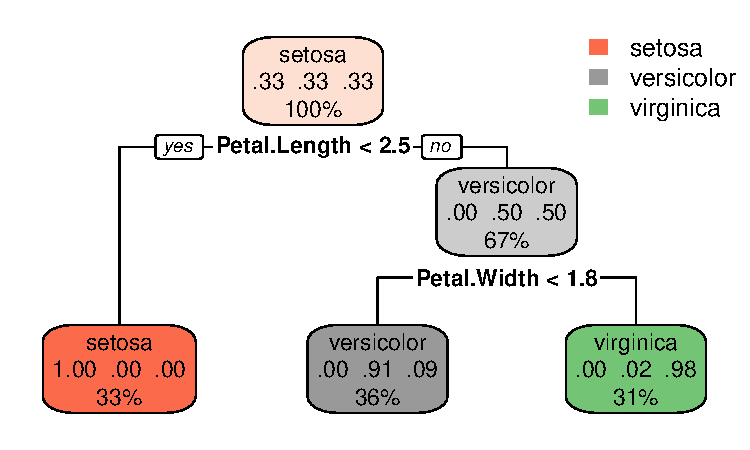
\includegraphics{ml_exercises_c1_treesbagging_files/figure-beamer/unnamed-chunk-8-1.pdf}

\end{frame}

\begin{frame}[fragile]{Solution - \texttt{rpart} - \texttt{iris} (III)}
\protect\hypertarget{solution---rpart---iris-iii}{}

\begin{enumerate}
[1)]
\setcounter{enumi}{2}
\tightlist
\item
  Prune the the using median complexity parameter (cp) associated to the
  tree.
\end{enumerate}

\begin{Shaded}
\begin{Highlighting}[]
\NormalTok{TP <-}\StringTok{ }\KeywordTok{prune}\NormalTok{(TREE2,}\DataTypeTok{cp=}\KeywordTok{median}\NormalTok{(TREE2}\OperatorTok{$}\NormalTok{cptable[,}\StringTok{'CP'}\NormalTok{]))}
\end{Highlighting}
\end{Shaded}

\begin{enumerate}
[1)]
\setcounter{enumi}{3}
\tightlist
\item
  Plot in the same window, the pruned and the original tree.
\end{enumerate}

\begin{Shaded}
\begin{Highlighting}[]
\KeywordTok{par}\NormalTok{(}\DataTypeTok{mfrow=}\KeywordTok{c}\NormalTok{(}\DecValTok{1}\NormalTok{,}\DecValTok{2}\NormalTok{))}
\KeywordTok{plot}\NormalTok{(TREE2);}\KeywordTok{text}\NormalTok{(TREE2,}\DataTypeTok{use.n=}\NormalTok{T)}
\KeywordTok{plot}\NormalTok{(TP);}\KeywordTok{text}\NormalTok{(TP,}\DataTypeTok{use.n=}\NormalTok{T)}
\end{Highlighting}
\end{Shaded}

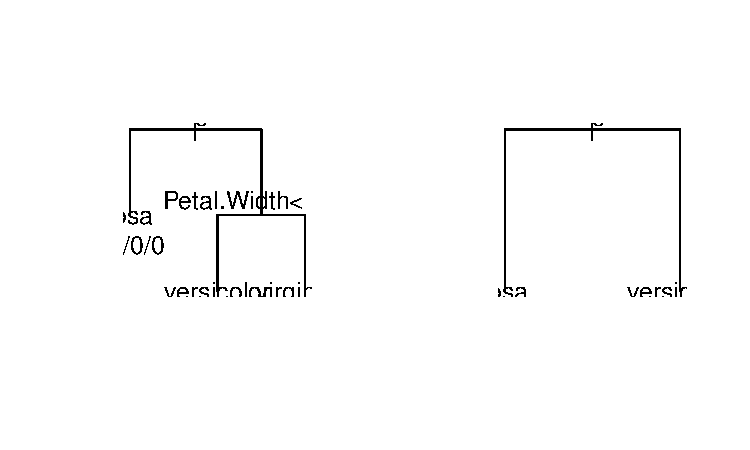
\includegraphics{ml_exercises_c1_treesbagging_files/figure-beamer/unnamed-chunk-10-1.pdf}

\end{frame}

\begin{frame}[fragile]{Solution - \texttt{rpart} - \texttt{iris} (IV)}
\protect\hypertarget{solution---rpart---iris-iv}{}

\begin{enumerate}
[1)]
\setcounter{enumi}{4}
\tightlist
\item
  In which terminal nodes is clasified each observations of iris?
\end{enumerate}

\begin{Shaded}
\begin{Highlighting}[]
\NormalTok{TREE2}\OperatorTok{$}\NormalTok{where}
\end{Highlighting}
\end{Shaded}

\begin{verbatim}
##   1   2   3   4   5   6   7   8   9  10  11  12  13  14  15  16  17  18 
##   2   2   2   2   2   2   2   2   2   2   2   2   2   2   2   2   2   2 
##  19  20  21  22  23  24  25  26  27  28  29  30  31  32  33  34  35  36 
##   2   2   2   2   2   2   2   2   2   2   2   2   2   2   2   2   2   2 
##  37  38  39  40  41  42  43  44  45  46  47  48  49  50  51  52  53  54 
##   2   2   2   2   2   2   2   2   2   2   2   2   2   2   4   4   4   4 
##  55  56  57  58  59  60  61  62  63  64  65  66  67  68  69  70  71  72 
##   4   4   4   4   4   4   4   4   4   4   4   4   4   4   4   4   5   4 
##  73  74  75  76  77  78  79  80  81  82  83  84  85  86  87  88  89  90 
##   4   4   4   4   4   4   4   4   4   4   4   4   4   4   4   4   4   4 
##  91  92  93  94  95  96  97  98  99 100 101 102 103 104 105 106 107 108 
##   4   4   4   4   4   4   4   4   4   4   5   5   5   5   5   5   4   5 
## 109 110 111 112 113 114 115 116 117 118 119 120 121 122 123 124 125 126 
##   5   5   5   5   5   5   5   5   5   5   5   4   5   5   5   5   5   5 
## 127 128 129 130 131 132 133 134 135 136 137 138 139 140 141 142 143 144 
##   5   5   5   4   5   5   5   4   4   5   5   5   5   5   5   5   5   5 
## 145 146 147 148 149 150 
##   5   5   5   5   5   5
\end{verbatim}

\end{frame}

\begin{frame}[fragile]{Solution - \texttt{rpart} - \texttt{iris} (V)}
\protect\hypertarget{solution---rpart---iris-v}{}

\begin{enumerate}
[1)]
\setcounter{enumi}{5}
\tightlist
\item
  Which species has a flower of \texttt{Petal.Length} greater than 2.45
  and \texttt{Petal.Width} less than 1.75.
\end{enumerate}

\begin{Shaded}
\begin{Highlighting}[]
\KeywordTok{print}\NormalTok{(}\StringTok{'versicolor'}\NormalTok{)}
\end{Highlighting}
\end{Shaded}

\begin{verbatim}
## [1] "versicolor"
\end{verbatim}

\end{frame}

\end{document}
